\chapter{Marco Conceitual do Curso}\label{sec:marco_conceitual}

% O marco conceitual do curso define o perfil do egresso. 
% helio - sugestão
% O egresso do curso de Bacharelado em Ciência da Computação da UFSCar, campus de São Carlos, possui sólida formação em Computação e é apto a projetar, implementar e gerenciar sistemas computacionais de propósito geral, sistemas de software, sistemas embarcados e aplicações científicas e gerenciais em diferentes domínios de aplicação. Além disso, o perfil do egresso leva em conta as necessidades de infraestrutura e aplicações regionais. 

Esta seção visa cobrir aspectos relacionados com o perfil do egresso deste curso. Para isso, inicialmente são apresentados os perfis genéricos dos principais cursos da área da computação; Ciência da Computação, Engenharia da Computação, Sistemas de Informação e Engenharia de Software. Logo após, apresenta-se um detalhamento que é específico do egresso do Bacharelado em Ciência da Computação da UFSCar, campus São Carlos.

\section{Perfis Genéricos da Área da Computação}

De acordo com a resolução Nro 5 de 16 de Novembro de 2016 \cite{SBC-Diretrizes}, os egressos dos cursos de computação são diferenciados de acordo com as habilidades e competências que eles devem possuir. Assim, almeja-se que os egressos desses cursos apresentem as seguintes habilidades/competências:

\textbf{Ciência da Computação:}

I - Sólida formação em Ciência da Computação e Matemática que os capacitem a: (i) construir aplicativos de propósito geral, ferramentas e infraestrutura de
software de sistemas de computação e de sistemas embarcados, (2) a gerar conhecimento científico e inovação e (3) %que os incentivem 
a estender suas competências à medida que a área se desenvolve;

II - Visão global e interdisciplinar de sistemas com o entendimento de que esta visão transcende os detalhes de implementação dos vários componentes e os conhecimentos dos domínios de aplicação;

III - Conhecimento sobre a estrutura dos sistemas de computação e os processos
envolvidos na sua construção e análise;

IV - Domínio dos fundamentos teóricos da área de Computação e como eles
influenciam a prática profissional;

V - Capacidade de agir de forma reflexiva na construção de sistemas de computação, compreendendo o seu impacto direto ou indireto sobre as pessoas e a sociedade;

VI - Capacidade de criar soluções, individualmente ou em equipe, para
problemas complexos caracterizados por relações entre domínios de conhecimento e de aplicação;

VII - Capacidade de reconhecer o caráter fundamental da inovação e da criatividade com a compreensão das perspectivas de negócios e oportunidades relevantes.

\textbf{Engenharia da Computação:}

I - Sólida formação em Ciência da Computação, Matemática e
Eletrônica visando à análise e ao projeto de sistemas de computação, incluindo sistemas voltados à automação e controle de processos industriais e comerciais, sistemas e
dispositivos embarcados, sistemas e equipamentos de telecomunicações e equipamentos de instrumentação eletrônica;

II - Conhemimento sobre os direitos e as propriedades intelectuais inerentes à produção e à utilização de sistemas de computação;

III - Capacidade de agir de forma reflexiva na construção de sistemas de computação, compreendendo o seu impacto direto ou indireto sobre as pessoas e a sociedade;

IV - Entendimento sobre o contexto social no qual a Engenharia é praticada, bem como os efeitos dos projetos de Engenharia na sociedade;

V - Capacidade de considerar sobre os aspectos econômicos, financeiros, de gestão e de qualidade, associados a novos produtos e organizações;

VI - Capacidade de reconhecer o caráter fundamental da inovação e da criatividade com a compreensão das perspectivas de negócios e oportunidades relevantes.

\textbf{Engenharia de Software:}

I - Sólida formação em Ciência da Computação, Matemática e
Produção, visando a criação de sistemas de software de alta qualidade de maneira
sistemática, controlada, eficaz e eficiente que levem em consideração questões éticas, sociais, legais e econômicas;

II - Capacidade de criar, individualmente ou em equipe, soluções para
problemas complexos caracterizados por relações entre domínios de conhecimento e de aplicação;

III - Capacidade de agir de forma reflexiva na construção de software,
compreendendo o seu impacto direto ou indireto sobre as pessoas e a sociedade;

IV - Entendimento sobre o contexto social no qual a construção de Software é praticada, bem como os efeitos dos projetos de software na sociedade;

V - Capacidade de compreender os aspectos econômicos e financeiros, associados a novos produtos e organizações;

VI - Capacidade de reconheer o caráter fundamental da inovação e da criatividade com a compreensão das perspectivas de negócios e oportunidades relevantes.

\textbf{Sistemas de Informação:}

I - Sólida formação em Ciência da Computação, Matemática e
Administração visando o desenvolvimento e a gestão de soluções baseadas em
tecnologia da informação para os processos de negócio das organizações de forma que elas atinjam efetivamente seus objetivos estratégicos de negócio;

II - Capacidade de determinar os requisitos, de desenvolver, de evoluir e de administrar os
sistemas de informação das organizações, assegurando que elas tenham as informações
e os sistemas de que necessitam para prover suporte a suas operações e obter vantagem competitiva;

III - Capacidade de inovar, planejar e gerenciar a infraestrutura de tecnologia da informação em organizações, bem como desenvolver e evoluir sistemas de informação para uso em processos organizacionais, departamentais e/ou individuais;

IV - Capacidade de escolher e configurar equipamentos, sistemas e programas para a solução de problemas que envolvam a coleta, processamento e disseminação de informações;

V - Entendimento sobre o contexto, envolvendo as implicações organizacionais e sociais, no qual as soluções de sistemas de informação são desenvolvidas e implantadas;

VI - Capacidade de compreender os modelos e as áreas de negócios, atuando como agentes de mudança no contexto organizacional;

VII - %Possam desenvolver 
Pensamento sistêmico que permita analisar e entender os problemas organizacionais

\section{Perfil do Egresso deste Curso}

A sólida formação teórica e técnica que este curso oferece, combinada com possibilidades de aprofundamento em diversas áreas, faz com que o egresso deste curso exiba três habilidades/competências que o caracterizam. 

A primeira é a capacidade de desenvolver soluções computacionais eficientes para os mais diversos tipos de problemas do cotidiano. Isso o habilita tanto a atuar em empresas nacionais e multinacionais da área de tecnologia, podendo assumir as mais variadas posições de emprego existentes, quanto a seguir uma carreira empreendedora, criando sua própria empresa. 

A segunda é a aptidão para seguir carreira científica, realizando mestrado, doutorado, pós-doutorado, e tornando-se pesquisador em universidades e/ou centros de pesquisa nacionais e internacionais. Essa linha de atuação permite que o egresso possa contribuir para a evolução da própria área de ciência da computação.  

A terceira é a capacidade de trabalhar eticamente em equipes, sabendo lidar com as diferenças de opiniões e respeitando diferentes pontos de vista, e sempre sabendo colocar suas posições educadamente. 


Atualmente, as empresas necessitam de profissionais habilitados para lidar com a grande quantidade de tecnologias que surgem diariamente na área da computação. Dessa forma, o egresso do Bacharelado em Ciência da Computação possui aptidões que lhe permitem atuar nos seguintes setores: i) instituições de ensino ou pesquisa, ii) organizações envolvidas com a produção de software ou hardware, iii) organizações em que software ou hardware é produto de apoio a suas atividades principais e iv) organizações que atuam na área de infraestrutura computacional. Além disso, o egresso está apto a empreender e gerar conhecimento científico e inovação, estendendo suas competências à medida que a área evolui~\cite{SBC-Diretrizes}. 

Vale ressaltar que as competências e habilidades adquiridas pelo egresso são também adaptáves a novas demandas que o mercado de trabalho local e regional apresentem. Essa adaptabilidade é obtida por meio do aprendizado de fundamentos e conceitos básicos, que são independentes das tecnologias e métodos atualmente em uso.

A seguir são apresentados os resultados esperados para os processos de aprendizagem e formação proporcionados pelo curso.

\section{Aptidões Específicas da Formação}

\subsection{Competências para Resolução de Problemas}

% helio - o egresso estará ou está?
O egresso do curso de Bacharelado em Ciência da Computação estará apto a:

\begin{itemize}
\begin{onehalfspace}
\item Resolver problemas matemáticos e lógicos relacionados à computação;
\item Resolver problemas relacionados a aspectos tecnológicos em computação;
\item Identificar problemas computacionalmente intratáveis e insolúveis, e possivelmente propor soluções aproximadas;
\item Resolver problemas envolvendo soluções computacionais aplicadas a outras áreas do conhecimento humano;
\item Identificar questões éticas, sociais e legais na área da computação, e consequentemente buscar soluções não conflitantes com essas questões. 
\end{onehalfspace}
\end{itemize}


\subsection{Competências para Compreensão de Conteúdos}

% helio - será ou é capaz?
Usando o conhecimento adquirido durante o curso de Bacharelado em Ciência da Computação o egresso será capaz de:

\begin{itemize}
\begin{onehalfspace}

\item Compreender e aplicar uma ampla gama de princípios e ferramentas disponíveis para o cientista de computação, conforme abordado pela matriz curricular; 
\item Aplicar seu senso cr\'itico de forma abrangente em diversos campos mais aprofundados da ciência da computação, permitindo o eventual aprimoramento desses campos em estudos de pós-graduação;
\item Aplicar seus conhecimentos sobre metodologias de pesquisa, permitindo o engajamento em atividades de pesquisa científica dentro e fora da academia;
\item Reconhecer e valorizar atributos de qualidade, responsabilidades profissionais e éticas do profissional de computação.
\end{onehalfspace}
\end{itemize}

\subsection{Competências para Desenvolvimento e Condução de Projetos}

No que diz respeito ao projeto de sistemas  computacionais, o egresso do curso de Bacharelado em Ciência da Computação será capaz de:

\begin{itemize}
\begin{onehalfspace}
\item Elaborar e conduzir projetos acadêmicos e profissionais na área de ciência da computação;
\item Projetar e programar sistemas de software e hardware;
\item Apresentar soluções computacionais a uma equipe, arguindo sobre as vantagens e desvantagens da solução; 
\item Coordenar o processo de desenvolvimento de software, utilizando metodologias adequadas; 
\item Construir um plano de negócios na área de computação; 
\item Gerenciar equipes de forma a obter bons níveis de produtividade e também possuir comportamento adequado ao participar de equipes, cooperando com os demais membros.

\end{onehalfspace}
\end{itemize}


\section{Aptidões Gerais da Formação}

\subsection{Habilidades Práticas}
No que diz respeito às habilidades práticas, o egresso do curso de Bacharelado em Ciência da Computação será capaz de:

\begin{itemize}
\begin{onehalfspace}
\item Planejar e realizar projetos individuais de pequeno ou grande porte;
\item Elaborar relatórios técnicos e apresentá-los com competência, em formato escrito ou oral;
\item Conduzir apresentações técnicas adequadas para o tempo, lugar e público;
\item Usar a literatura científica de forma eficaz, bem como os recursos disponíveis na Web;
\item Utilizar ferramentas computacionais apropriadas para dar suporte à condução de projetos;
\item Aplicar conhecimentos de informática em ambiente comercial, industrial ou de pesquisa;
\item Demonstrar iniciativa, inovação e autogestão na condução de projetos;
\item Integrar as competências previamente adquiridas e aplicá-las a novas situações.
\end{onehalfspace}
\end{itemize}

\subsection{Competências para o Trabalho em Equipe}
No que diz respeito ao trabalho em equipe, o egresso do Bacharelado em Ciência da Computação será capaz de:

% helio - puxa, será que estamos promovendo o aprendizado efetivo de todos esses quesitos?

\begin{itemize}
\begin{onehalfspace}
\item Demonstrar capacidade de trabalho em grupo;
\item Trabalhar eficazmente com e para outras pessoas;
\item Liderar equipes;
\item Comunicar-se de forma efetiva com pessoas da área de computação e de outras áreas, em qualquer nível hierárquico;
\item Encontrar o equilíbrio entre a autossuficiência e a busca por ajuda;
\item Realizar funções técnicas e administrativas dentro de uma equipe de trabalho;
\item Mostrar responsabilidade para o cumprimento de prazos e metas de custos;
\item Desenvolver planos de carreira e objetivos pessoais.\\
\end{onehalfspace}
\end{itemize}

% \helena{}{A Figura~\ref{fig:perfil_egresso} traz uma ilustração gráfica do perfil do egresso do curso de Bacharelado em Ciência da Computação.}

% \begin{figure}[htb!]
%     \centering
%     %\includegraphics{}
%     \helenacomentario{Não sou boa para fazer figuras. Uma sugestão aqui seria fazer um diagrama de Venn com as principais aptidões citadas nas subseções anteriores :o(}
%     \danielcomentario{Precisa de figura mesmo? Não consigo pensar em uma representação visual que seja necessária aqui.}
%     \caption{\mario{Apresentação}{Representação} gráfica do perfil do egresso do curso de \mario{Bacharelado em}{} Ciência da Computação}
%     \label{fig:perfil_egresso}
% \end{figure}

A Figura~\ref{fig:perfil_egresso} traz uma ilustração gráfica do perfil do egresso do Bacharelado em Ciência da Computação. A figura destaca três grandes conceitos que são base para o curso: Núcleos de Conhecimento, Linhas de Formação e Atividades Complementares. 

Os Núcleos de Conhecimento são componentes curriculares abstratos que agrupam disciplinas relacionadas. Este curso está dividido em 7 Núcleos de Conhecimento, como pode ser visto na Figura~\ref{fig:perfil_egresso}.A sobreposição existente entre alguns Núcleos de Conhecimento revela a multidisciplinaridade existente. Em nível mais granular, essa multidiscipinaridde é implementada por meio de projetos comuns entre disciplinas e outros mecanismos pedagógicos adequados. 

A figura também ressalta o conceito de Linhas de Formação, mostrando que assim que o estudante foi capacitado na área fundamental e base do curso, ele poderá, a critério próprio, se aprofundar em determinados temas. Este curso oferece 10 Linhas de Formação, cujos nomes encontram-se em cada uma das setas que representam as linhas de formação.

Em paralelo a este cenário pedagógico que mescla capacitação em áreas fundamentais e flexibilização para formações mais específicas, encontram-se as atividades complementares, representadas pelo funil do lado direito da figura. Essas, por sua vez, visam complementar a formação que o estudante recebe em sala de aula, expondo-o a situações e experiências que fortalecem o desenvolvimento de competências e habilidades diversificadas. Essas experiências tornam o egresso do curso em um profissional totalmente preparado para o ambiente real de trabalho, seja na indústria ou na academia. 

Detalhes mais específicos sobre os Núcleos de Conhecimento, Linhas de Formação e Atividades encontram-se no decorrer deste documento. 

\begin{figure}[htb!]
    \centering
    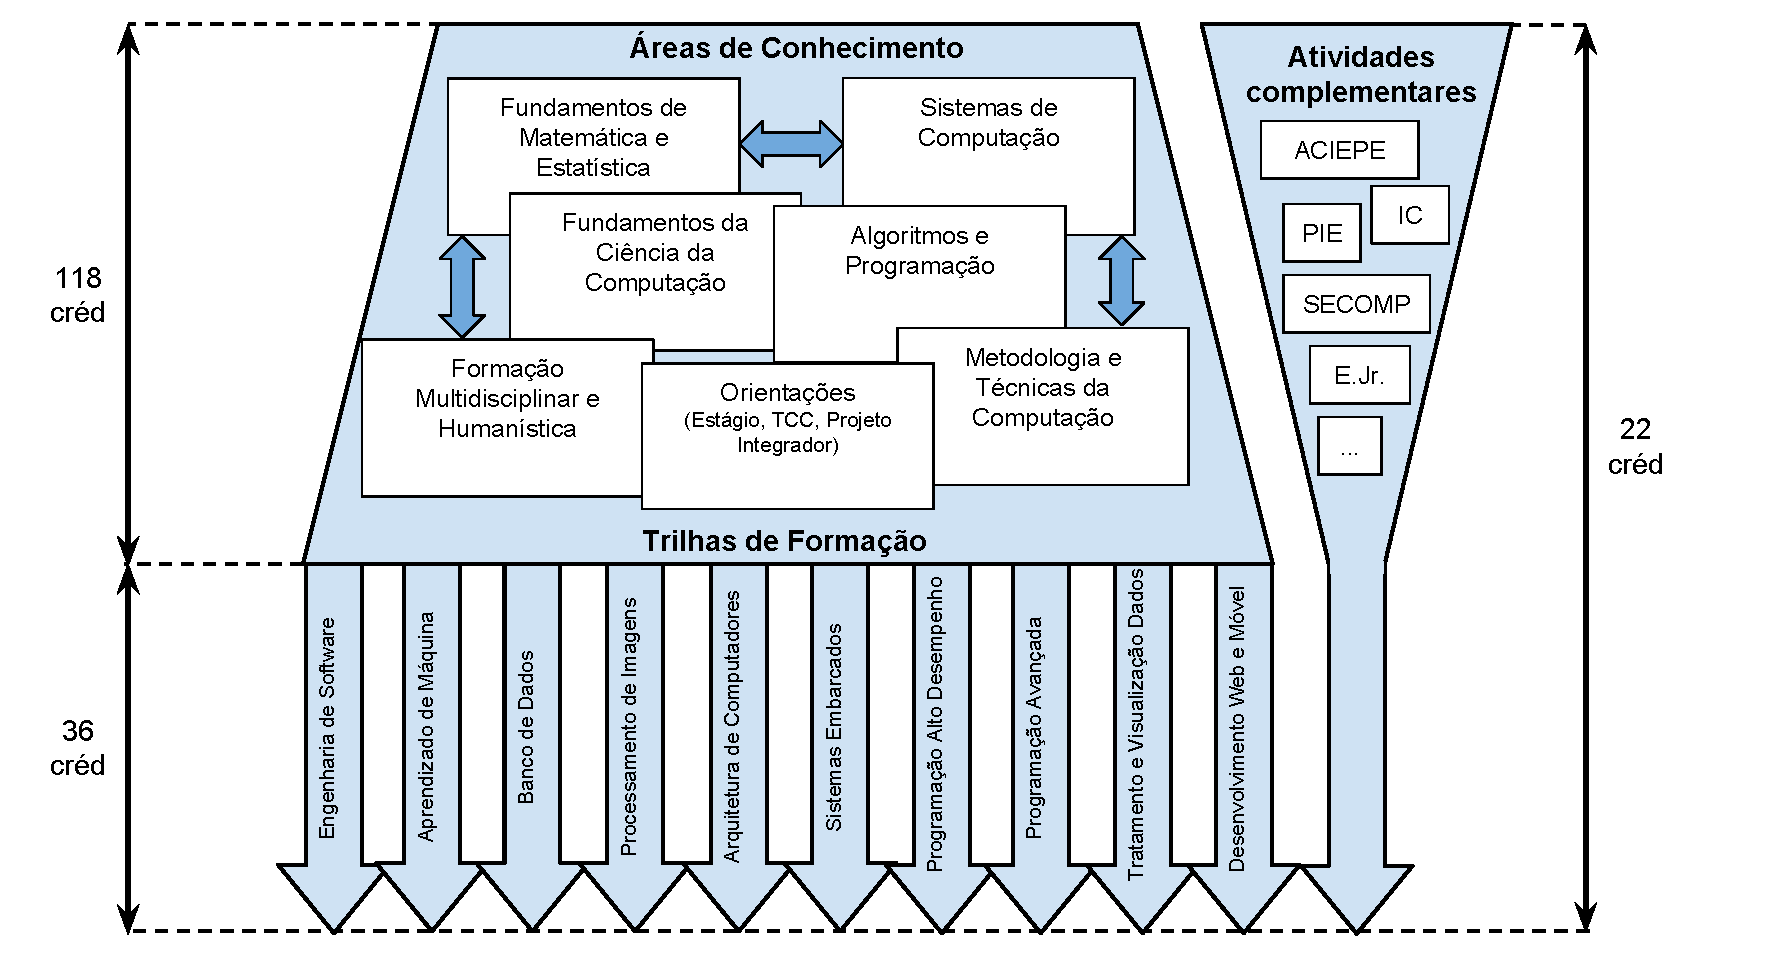
\includegraphics[width=\columnwidth]{bcc/imagens/perfil_egresso.pdf}
    \caption{Representação gráfica do perfil do egresso do curso de Ciência da Computação}
    \label{fig:perfil_egresso}
\end{figure}